\documentclass[conference]{IEEEtran}

% --- packages (standalone figs only) ---
\usepackage{graphicx}
\usepackage{tikz}
\usepackage{pgfplots}
\pgfplotsset{compat=1.18}
\usetikzlibrary{arrows.meta,positioning}
\usepackage{subcaption} % Fig.3 横並び
\pagestyle{empty}

% 少しだけキャプション間隔を詰める(ページ節約)
\makeatletter
\setlength{\abovecaptionskip}{5pt}
\setlength{\belowcaptionskip}{2pt}
\makeatother

\begin{document}

% ===== Title =====
\title{\Large\bfseries Supplementary Figures and Tables for\\
``FeFET CMOS 0.18~$\mu$m Integration Study''}
\author{}
\maketitle

% ================= Page 1: Process Integration =================
% --- Fig.1 (Process flow, vertical TikZ) ---
\begin{figure}[!t]
\centering
\begin{tikzpicture}[
  node distance=4.5mm,
  stage/.style={draw,rounded corners,minimum width=35mm,
                minimum height=6mm,align=center,font=\footnotesize},
  arr/.style={-{Stealth},thick},
  ann/.style={font=\scriptsize}
]
\node[stage] (act)  {Active / Isolation};
\node[stage,below=of act] (vt)  {V\!T Adjust / Well};
\node[stage,below=of vt]  (poly) {Poly Gate Definition};
\node[stage,below=of poly] (ldd)  {LDD / Spacer};
\node[stage,below=of ldd]  (imp)  {S/D Implant};
\node[stage,below=of imp]  (sal)  {Co Salicide \& Lamp Anneal};
\node[stage,below=of sal]  (fegate)  {FeFET Gate-Last: IL/FE/CAP (ALD) + TiN (PVD/ALD)};
\node[stage,below=of fegate]  (rta)  {Crystallization RTA (450--500\,\si{\celsius}) + FGA (350\,\si{\celsius})};
\node[stage,below=of rta]  (ild)  {ILD + Vias + BEOL};

\draw[arr] (act) -- (vt) -- (poly) -- (ldd) -- (imp) -- (sal) -- (fegate) -- (rta) -- (ild);

% dashed bracket to highlight FeFET module
\node[draw,dashed,very thick,rounded corners,fit=(fegate) (rta),inner sep=3mm,
      label={[ann]right:\textbf{FeFET Gate-Last Module}}] {};

% note box
\node[draw,rounded corners,align=left,font=\scriptsize,anchor=east,
      right=12mm of fegate] (note) {Added masks: +1 (FE metal gate)\\
Anneal: BEOL furnace (no mask)\\
TiN: long-throw/collimated PVD};
\draw[arr] (note.west) -- (fegate.east);
\end{tikzpicture}
\caption{Placement of the FeFET gate-last module within the 0.18~$\mu$m CMOS baseline (vertical layout).}
\label{fig:flow}
\end{figure}

\vspace{1em} % 図と表の間隔を確保

% --- Table I (Added masks) ---
\begin{table}[!t]
\centering
\caption{Added masks / process steps relative to baseline logic.}
\label{tab:masks}
\begin{tabular}{|c|c|l|}
\hline
\textbf{Step} & \textbf{Mask} & \textbf{Comment} \\ \hline
FE metal gate & +1 & Reuse analog option route \\ 
FE anneal     & 0  & Performed in BEOL furnace (no extra mask) \\ \hline
\end{tabular}
\end{table}

% ================= Page 2: Reliability Data =================
\section*{Figures and Tables (Reliability Data)}

% --- Fig.2: Endurance ---
\begin{figure}[!t]
\centering
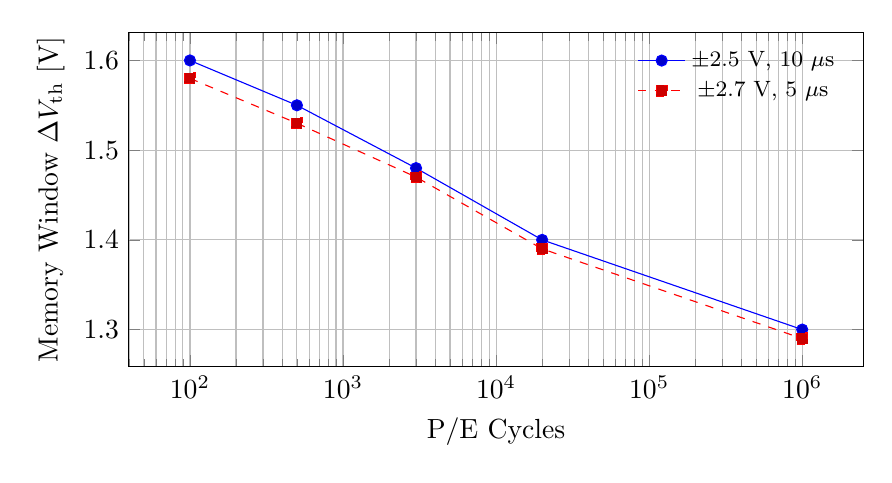
\begin{tikzpicture}
\begin{axis}[
  width=0.90\linewidth, height=0.48\linewidth,
  xlabel={P/E Cycles}, xmode=log, log basis x=10,
  ylabel={Memory Window $\Delta V_{\mathrm{th}}$ [V]},
  grid=both,
  legend style={draw=none, fill=none, font=\footnotesize},
]
\addplot+[mark=*] coordinates {(1e2,1.60) (5e2,1.55) (3e3,1.48) (2e4,1.40) (1e6,1.30)};
\addlegendentry{$\pm 2.5$ V, 10 $\mu$s}
\addplot+[mark=square*, dashed] coordinates {(1e2,1.58) (5e2,1.53) (3e3,1.47) (2e4,1.39) (1e6,1.29)};
\addlegendentry{$\pm 2.7$ V, 5 $\mu$s}
\end{axis}
\end{tikzpicture}
\caption{Schematic endurance behavior of HZO-FeFETs in a 0.18~$\mu$m flow.}
\end{figure}

% --- Fig.3: Wake-up & Retention (横並び) ---
\begin{figure}[!t]
\centering
\begin{subfigure}[t]{0.48\linewidth}
\centering
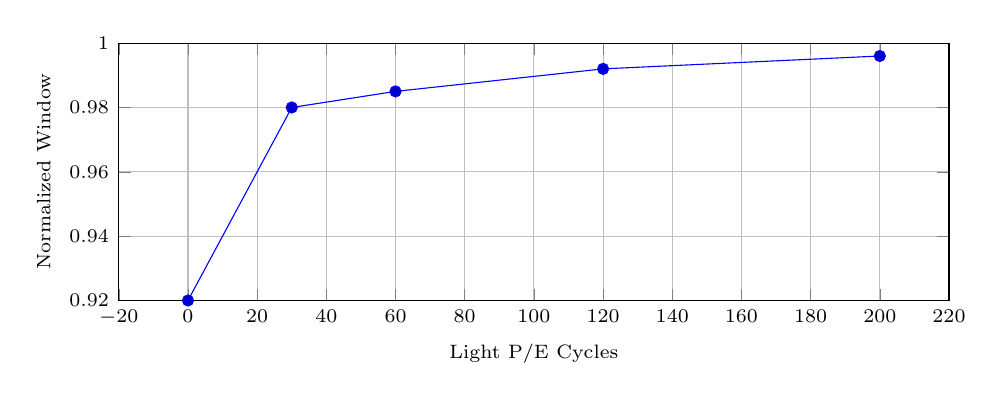
\begin{tikzpicture}
\begin{axis}[
  width=\linewidth, height=0.40\linewidth,
  xlabel={Light P/E Cycles}, ylabel={Normalized Window},
  grid=both, ymin=0.92, ymax=1.00,
  tick label style={font=\scriptsize},
  label style={font=\scriptsize},
]
\addplot+[mark=*] coordinates {(0,0.92) (30,0.98) (60,0.985) (120,0.992) (200,0.996)};
\end{axis}
\end{tikzpicture}
\caption{Wake-up (early cycles).}
\end{subfigure}\hfill
\begin{subfigure}[t]{0.48\linewidth}
\centering
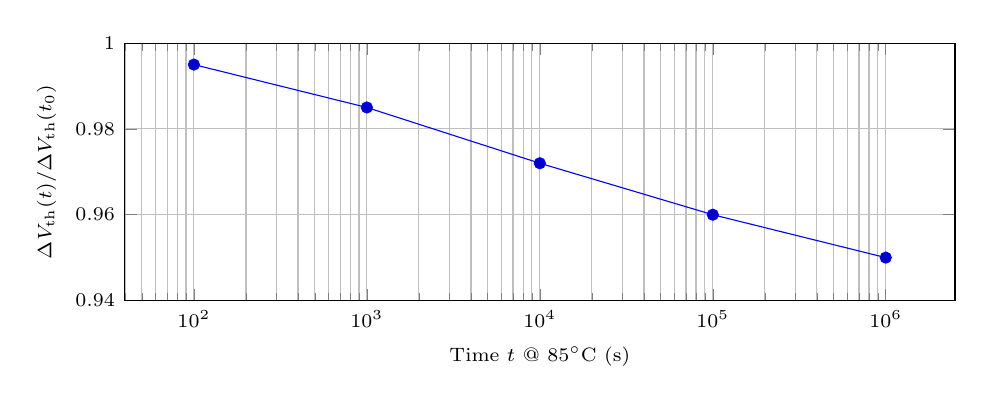
\begin{tikzpicture}
\begin{axis}[
  width=\linewidth, height=0.40\linewidth,
  xmode=log, log basis x=10, grid=both,
  xlabel={Time $t$ @ 85$^\circ$C (s)},
  ylabel={$ \Delta V_{\mathrm{th}}(t)/\Delta V_{\mathrm{th}}(t_0)$},
  tick label style={font=\scriptsize},
  label style={font=\scriptsize},
  ymin=0.94, ymax=1.00,
]
\addplot+[mark=*] coordinates {(1e2,0.995) (1e3,0.985) (1e4,0.972) (1e5,0.960) (1e6,0.950)};
\end{axis}
\end{tikzpicture}
\caption{Retention projection.}
\end{subfigure}
\caption{Wake-up and retention behaviors at 85$^\circ$C.}
\end{figure}

% --- Fig.4: TDDB Weibull ---
\begin{figure}[!t]
\centering
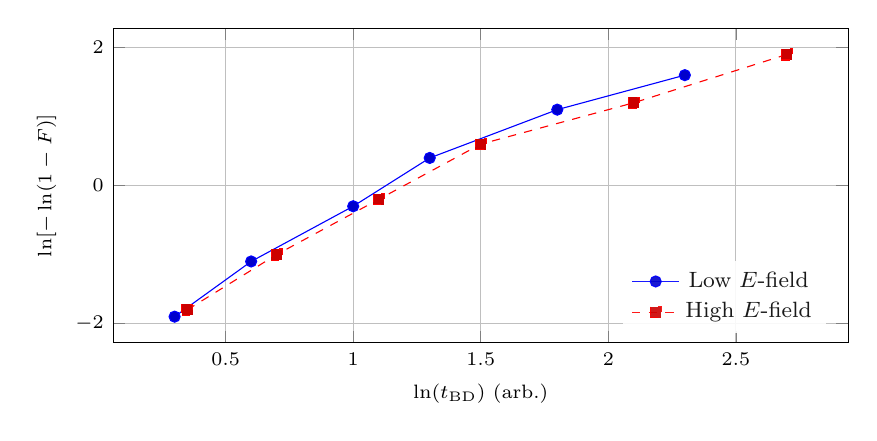
\begin{tikzpicture}
\begin{axis}[
  width=0.90\linewidth, height=0.46\linewidth,
  xlabel={$\ln(t_{\mathrm{BD}})$ (arb.)},
  ylabel={$\ln[-\ln(1-F)]$},
  grid=both,
  legend pos=south east,
  legend style={fill=white, draw=none, opacity=0.9, font=\footnotesize},
  tick label style={font=\scriptsize},
  label style={font=\scriptsize},
]
\addplot+[mark=*] coordinates {(0.3,-1.9) (0.6,-1.1) (1.0,-0.3) (1.3,0.4) (1.8,1.1) (2.3,1.6)};
\addlegendentry{Low $E$-field}
\addplot+[mark=square*, dashed] coordinates {(0.35,-1.8) (0.7,-1.0) (1.1,-0.2) (1.5,0.6) (2.1,1.2) (2.7,1.9)};
\addlegendentry{High $E$-field}
\end{axis}
\end{tikzpicture}
\caption{TDDB Weibull representation at two stress fields (illustrative).}
\end{figure}

\end{document}
